\Answer
Suppose we have a system of $N$ particles with number density $\rho$, thus the
box size will be

\begin{equation}
    L = \bigg( \frac{ N }{ \rho } \bigg)^{1 / 3}.
\end{equation}

If we want to impose the periodic boundary conditions (PBCs) here, we should adopt the
nearest image convention (NIC) or minimum image convention (MIC). What is an image? First,
we should emphasize that we could not do simulations in an infinitely large box (cell) in MD
simulations. The most common solution is to take one cell (we will call it ``center cell''
in the following text) to simulate and imagine an infinitive number of image cells
surrounding it, where each image cell is a replica of the center cell. The image cells can
reduce or eliminate boundary effects by providing every particle an equivalent surrounding
environment of particles as if it were in the bulk, no matter where they are in the center
cell.

\begin{figure}[h]
    \centering
    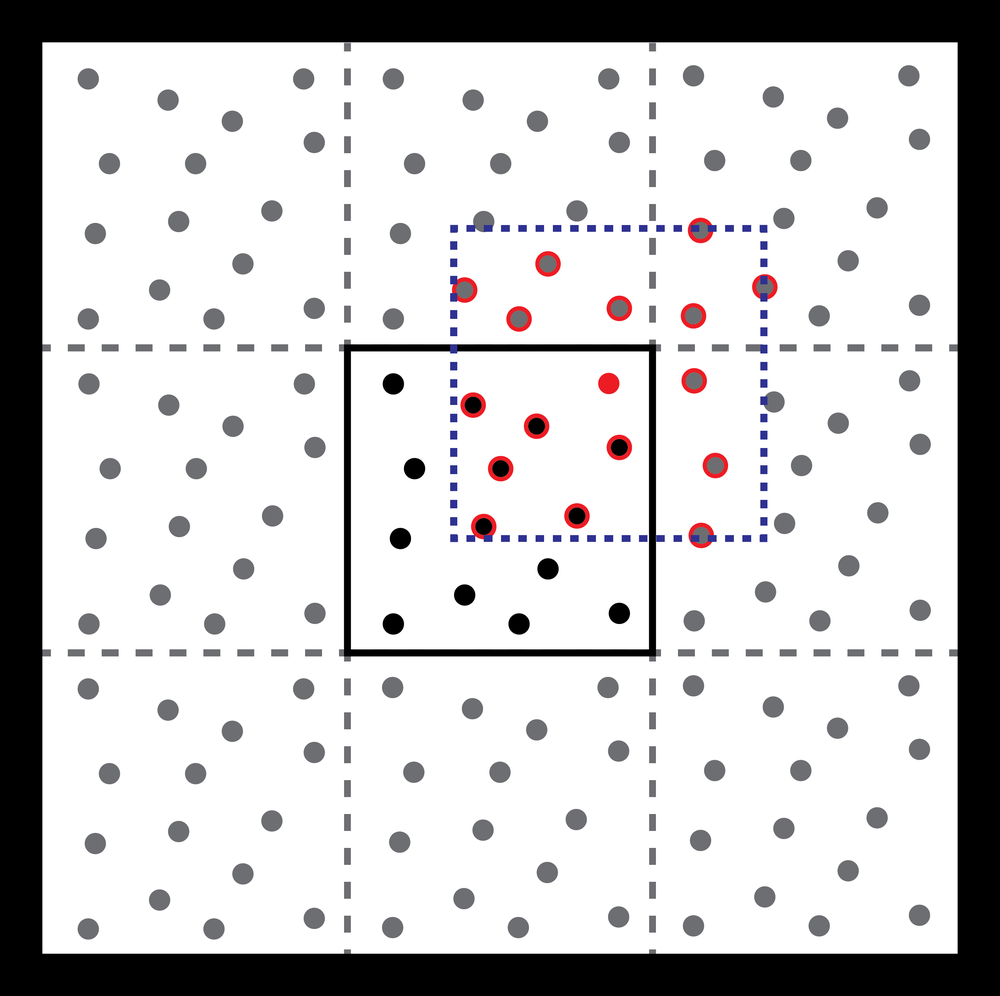
\includegraphics[width=0.5\textwidth]{nic}
    \caption{A center cell surrounded by $8$ more image cells with the same
        particles' relative locations and movements.}\label{fig:nic}
\end{figure}

When applying PBCs, particles near the edge of the cells often interact
with an image particle rather than a particle in the cell. For example, we can create the
situation shown below.
In Figure~\ref{fig:nic}, the black border box is our center cell, and the $8$ others are
its replica. The relative positions and velocities of the particles in these image cells
are exactly the same as their originals in the center cell. The red particle in the
upper left corner of the center cell only interacts with its neighbors: some of the
particles in the center cell plus some of the image particles in the image cells.
We call the box enclosing the red particle's neighbors a ``virtual image cell''.
The size of the virtual image cell (cutoff radius) is usually chosen as $L / 2$
of the center cell. That is, any particle which is more than $L / 2$ away from the
red particle in any direction is not included in the virtual image cell.
If the cutoff radius is larger than $L / 2$, it may lead to
unphysical self-interactions, sometimes called an artifact.

Another aspect of the PBCs is that when a particle hits a cell wall, instead of bouncing
back, it reappears on the other side of the cell (the topology of a torus), or we can
treat it as an image particle from an adjacent cell enters the current cell.
So the number of particles in a cell never increases or decreases in this case.

So how do we express the PBCs in mathematical and programming languages?
Suppose we have two particles, $a$ and $b$, and $a$ is the particle in which we
are interested. The vector pointing from $a$ to $b$ is the difference between
their positions:
%
\begin{equation}
    \bm{r} = \bm{r}_b - \bm{r}_a.
\end{equation}
%
For any component $r_\alpha$ of $\bm{r}$, where $\alpha = 1, 2, 3$, if its absolute value
is larger than $L / 2$, then we know $b$ is too far from $a$ to have effects on it,
so we should shift $b$ closer to $a$ in the corresponding dimension:
%
\begin{equation}
    \begin{cases}
        r_{b, \alpha} - L, & \text{if } r_\alpha > L / 2,                  \\
        r_{b, \alpha} + L, & \text{if } r_\alpha < -L / 2,                 \\
        r_{b, \alpha},     & \text{if } \lvert r_\alpha \rvert \leq L / 2,
    \end{cases}
\end{equation}
%
where $r_{b, \alpha}$ is the component of the position of particle $b$ in the
corresponding dimension.
The Julia code for the above procedure looks like Snippet \ref{lst:pbcs}:

\begin{algorithm}
    \caption{Find the nearest image of particle $b$ which can interact with particle $a$.}
    \label{lst:pbcs}
    \begin{juliacode}
        Δ𝐫 = b.position - a.position
        position = map(b.position, Δ𝐫) do rᵢ, Δrᵢ
            if Δrᵢ > L / 2
                rᵢ - L
            elseif Δrᵢ < -L / 2
                rᵢ + L
            else  # |Δrᵢ| <= L / 2
                rᵢ  # Do not shift
            end
        end
    \end{juliacode}
\end{algorithm}
